\chapter{Shapes}

Once you know how to show a dot on the screen, other shapes are easy. (If you don't, review chapter \ref{chapter:positions}.) Most mathematical shapes can be drawn on the screen. The classes to do that are in the green folder Esenthel Engine $\Rightarrow$ Math $\Rightarrow$ Shapes.

Not all available shapes are intended for display in 2D. Some classes, like \eeClass{Ball} and \eeClass{Tube}, are intended for 3D development. For now, we will focus on 2D shapes like \eeClass{Circle}, \eeClass{Edge} (line), \eeClass{Quad}, \eeClass{Rectangle} and \eeClass{Triangle}.

\section{Circle}
To draw a circle you need a radius(r) and a position(pos). The radius is a \eeClass{float}, the position a \eeClass{Vec2}. There is more than one way to pass these to a circle:

\begin{code}
// using the constructor, with r(float), pos.x(float), pos.y(float)
Circle c(0.1, 0, 0);

// using the constructor, with r(float), pos(Vec2)
Circle c(0.1, Vec2(0, 0));

// during the coarse of the application
c.set(0.1, 0, 0);
c.set(0.1, Vec2(0, 0));

// directly changing the variables
c.r = 0.1;
c.pos = Vec2(0, 0);
\end{code}

\subsection{Methods}
The set function aside, there are also methods available to retrieve the current area or perimeter, and to draw the circle on the screen.

\begin{code}
// retrieve area and perimeter
float a = c.area();
float b = c.perimeter();

// draw a blue circle on the screen
c.draw(BLUE);

// draw the perimeter only
c.draw(BLUE, false);
\end{code}

There's something remarkable about the \eeFunc{draw} method! It can be used with one as well as with two methods. To see how this is possible, look at the declaration of this method, which can be found at Esenthel Engine $\Rightarrow$ Math $\Rightarrow$ Shapes $\Rightarrow$ Circle:

\begin{code}
void draw(C Color & color, Bool fill = true, Int resolution = -1) C;
\end{code}

The first argument is a \eeClass{Color}. The second argument is a \eeClass{bool} named `fill'. You might suspect this means whether or not you desire to draw the circle as a perimeter or an area. And of course you're right. Only, the argument doesn't stop there: it has a value assigned ( = true). This is called a default value. If you agree with the default, you don't gave to explicitly pass true as an argument. Only when you don't agree, you will have to pass false.

\begin{note}
The third argument (resolution) is also optional. Experiment with several values to find out what is does. (Try values like 2, 3, 8, 14, \ldots)
\end{note}

\subsection{Math}
You can do math with circles. There are operators like \eeOpp{+=}, \eeOpp{-=}, \eeOpp{/=} and \eeOpp{*=}, which can be used to alter the radius or the position. How do you know which value will be altered? Well, if you add a float to a circle, the radius change. When you add a \eeClass{Vec2} this will later the position.

\begin{code}
Vec2 pos(0.1, 0);
Circle c(0.1, pos);

// move the circle 0.1 units to the right
c += pos;
// move the circle 0.2 units down
c -= Vec2(0, 0.2);
// double the radius
c *= 2;
\end{code}

\subsection{Excercises}
Recreate the folowing image by drawing circles on the screen. If you like a challenge, try creating a more fitting mouth with the method \eeFunc{drawPie}.

\begin{figure}[h]
\centering
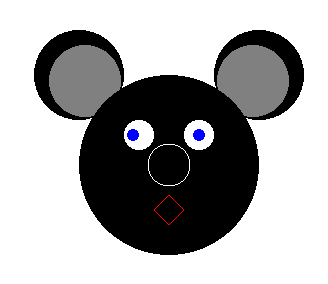
\includegraphics[width=0.4\linewidth]{../images/circle_exercise}
\caption[]{Pay attention to the eyes!}
\label{fig:pos2D}
\end{figure}

\section{Edge2}
An \eeClass{Edge2} is a line. Just as with \eeClass{Vec2}, the '2' is important. The code will still be valid when you use an \eeClass{Edge} instead of an \eeClass{Edge2}, but that class is intended for drawing in 3D instead. To define an \eeClas{Edge2}, you need two points (\eeClass{Vec2}), being the beginning and the end. Esenthel offers two methods to pass these to the object:

\begin{code}
Edge2 e1;
Edge2 e2;

// using newly created vectors ...
e1.set(Vec2(0, 0), Vec2(0.1, 0.1));

// ... or existing vectors
Vec2 pos1(0.3, 0.6);
Vec2 pos2(0.1, 0.2);
e1.set(pos1, pos2);

// set all x and y values as floats
e2.set(-0.4, 0.2, -0.7, 0.9;
\end{code}

\subsection{Methods}
An \eeClass{Edge2} provides several neat methods. The most obvious will be \eeFunc{draw()}:

\begin{code}
line1.draw(PURPLE    ); // draw a purple line
line2.draw(GREEN, 0.1); // draw a green line, with width 0.1
line3.draw(GREEN, RED); // draw a line that starts out green but fades to read
\end{code}

Other methods of interest are \eeFunc{center()}, \eeFunc{delta()}, \eeFunc{dir()} and \eeFunc{length()}. All of them can be found in $\Rightarrow$ Math $\Rightarrow$ Shapes $\Rightarrow$ Edge.

\subsection{Exercises}

The methods \eeFunc{Sin()} en \eeFunc{Cos()} allow you to retrieve the sine and cosine from any value. This is most fun when that value is the current time. The result over time is a value which moves smoothly between -1 and 1.

\begin{code}
float x = Sin(Time.curTime());
float y = Cos(Time.curTime());
\end{code}

\begin{enumerate}
\item The code above illustrates how to use the sine and cosine with the current time. Create an application which shows a line, starting from the middle of the screen towards the current value of sine and cosine for the x and y value of the ending.
\item Change the width of the line.
\item Make the line move at double speed.
\item Decrease the length of the line. 
\item \textit{(This will be a bit harder)} Try to create an analog watch.
\end{enumerate}

Take a look at Esenthel Engine $\Rightarrow$ Math $\Rightarrow$ Shapes $\Rightarrow$ Edge. Examine the method \eeFunc{lerp(float s)} vinden. This function needs an argument between zero and one, and return a position on the line.

\begin{enumerate}
\item Define an \eeClass{Edge2} and a \eeClass{float} with value zero.
\item In the init function, assign a start and end position to your line.
\item In the update function you increase the float with \eeClass{Time.d()}. When the float value is larger than 1, is should be assigned 0.
\item Draw the line in black with a width of 0.05. Construct a \eeClass{Vec2} with the result of \eeFunc{lerp()}. The argument of the method should be your float. Draw this point in red, also with a width of 0.05.
\end{enumerate}

Draw a triangle on the screen.

\section{Rect}
The last shape in the chapter is a rectangle: \eeClass{Rect}. You will end up using this shape quite a lot, because a rectangle happens to be the shape of most gui elements, like buttons, windows and images.

After the last exercise, you know that you need 3 positions to draw a triangle. Logic dictates a rectangle requires 4 positions, right? But there's one property of a rectangle that makes it a lot easier: all corners have an angle of 90\%. This means that when you pass the lower left corner and the upper right corner, there is enough information to find the two remaining corner positions.

\begin{figure}[h]
\centering
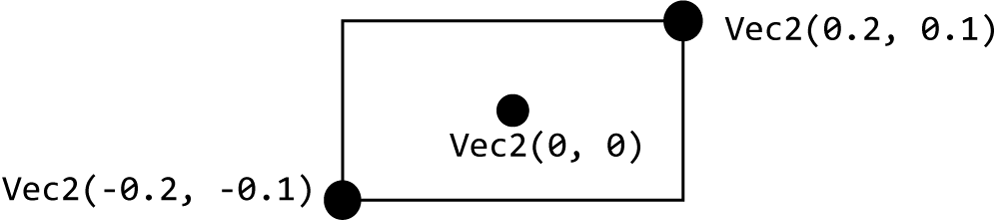
\includegraphics[width=0.8\linewidth]{../images/rectangle}
\caption[]{The corners of a rectangle}
\label{fig:rect}
\end{figure}

This means a rectangle can be created like this:

\begin{code}
Rect(Vec2(-0.2, -0.1), Vec2(0.2, 0.1)).draw(BLACK, false);
\end{code}

Zoals je ziet is er ook nu een draw functie, waarin het eerste argument de kleur is, en je daarna optioneel kan aangeven dat je de rechthoek niet wil vullen. Net zoals bij een edge heb je ook nu weer de mogelijkheid om de x- en y-co\"ordinaat afzonderlijk in te geven:

\begin{code}
Rect(-0.2, -0.1, 0.2, 0.1).draw(BLACK);
\end{code}

\subsection{A moving Rectangle}
If you want to draw an image on the screen, it will require a rectangle. As such, a rectangle will be the basis of almost every element on your screen. It will often come in handy to have a special class for movable rectangles. As an example, we'll create a rectangle which can be moved with the arrow keys.

Rectangles have one big disadvantage when you try to move them. Instead of a central position, both corners have to be moved. This is why we often use a \eeClass{Vec2} to remember the center position. As an extra, this class will remember its color.


\begin{code}
class movableRect {
  	Vec2 pos;
	Color color;
}
\end{code}


Deze class kunnen we uitbreiden met een create functie, een update functie en een draw functie. Via de create functie geef je de kleur en de startpositie door. De startpositie heeft een standaard waarde, dus wanneer je later de create functie gebruikt zonder een positie, dan staat de rechthoek in het midden van het scherm.

\begin{code}
void create(C Color & color, C Vec2 & pos = 0) {
  T.color = color;
	T.pos = pos;
}
\end{code}

\begin{note}
In deze functie staan nog enkele nieuwigheden. De ampersand geeft aan dat we color en pos als referentie doorgeven. De \eeFunc{C} betekent dat we de waarde niet zullen aanpassen. Je leert hierover meer in een van de volgende hoofdstukken. De letter \eeFunc{T} lost een praktisch probleem op. Zowel het functie-argument als de Color in de class zelf hebben als naam `color'. De compiler kan daarom niet weten wanneer je welke variabele bedoelt. Je zou ze beiden een verschillende naam kunnen geven, maar dat maakt de code moeilijker leesbaar. De elegante oplossing bestaat er in \eeFunc{T.} voor de variabele van de class toe te voegen. De T staat voor `this' en daarmee bedoelen we `deze class'. De versie zonder \eeFunc{T.} is bijgevolg de variabele die we als functieargument doorgeven.
\end{note}

In de update functie kunnen we de positie wijzigen via de pijltjestoetsen. Deze code heb je reeds gezien in hoofdstuk \ref{chapter:keyboardInteractie}.

\begin{code}
void update() {
	if(Kb.b(KB_LEFT )) pos.x -= Time.d();
	if(Kb.b(KB_RIGHT)) pos.x += Time.d();
	if(Kb.b(KB_UP   )) pos.y += Time.d();
	if(Kb.b(KB_DOWN )) pos.y -= Time.d();
}
\end{code}


Tot slot is er een draw functie nodig. Het is pas op deze plaats dat we, tijdelijk, een rechthoek maken. In dit geval is dat het meest praktisch, maar dat hoeft niet altijd zo te zijn. Het zou bijvoorbeeld kunnen dat je in de update functie wil controleren of de rechthoek iets raakt. In zo'n geval zou je waarschijnlijk ook een \eeClass{Rect} aan je class toevoegen.

\begin{code}
void draw() {
  Rect(pos - Vec2(0.2, 0.1), pos + Vec2(0.2, 0.1)).draw(color);
}
\end{code}

Zoals je ziet gebruiken we de positie `pos' bij het maken van de rechthoek. Die is namelijk het middelpunt. Aangezien we de hoeken linksonder en rechtsboven nodig hebben bij het maken van een rechthoek, kunnen we eenvoudig een waarde respectievelijk aftrekken en optellen. We zouden deze class nog wat meer flexibel kunnen maken door een `size' te onthouden.

Omdat dit de eerste maal is dat we een volledige class uitwerken in esenthel krijg je ze hieronder nog eens helemaal te zien. Let ook op de keywords public en private. Die zijn later belangrijk als je je code overzichtelijk wil houden.

\begin{code}
class movableRect {
private:
  Vec2 pos, size;
	Color color;
	
public:
  void create(C Color & color, C Vec2 & pos = 0, C Vec2 & size = Vec2(0.1, 0.1)) {
	  T.color = color;
		T.pos   = pos  ;
		T.size  = size ;
	}
	
	void update() {
		if(Kb.b(KB_LEFT )) pos.x -= Time.d();
		if(Kb.b(KB_RIGHT)) pos.x += Time.d();
		if(Kb.b(KB_UP   )) pos.y += Time.d();
		if(Kb.b(KB_DOWN )) pos.y -= Time.d();
	}
	
	void draw() {
		Rect(pos - size, pos + size).draw(color);
	}
}
\end{code}
	
\subsection{Oefeningen}

\begin{enumerate}
\item Maak in een programma de volgende afbeelding na:

\begin{figure}[h]
\centering
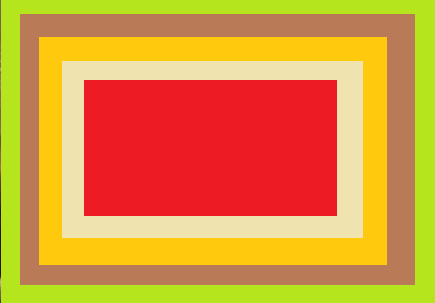
\includegraphics[width=0.4\linewidth]{../images/nested_rectangles}
\caption[]{Rechthoeken}
\label{fig:nested_rect}
\end{figure}

\item Voeg een roze vierkant toe van de class \eeClass{movableRect} die we hierboven voorstelden.
\item \textbf{(Uitbreiding)} Zorg dat het vierkant niet buiten het scherm kan bewegen.
\end{enumerate}

\section{Cuts}

Een functie die je vaak gebruikt in verband met shapes is \eeFunc{Cuts}. Er bestaan heel veel varianten op deze functie, maar de betekenis is steeds dezelfde: raken twee objecten mekaar of niet? Zo kan je controleren of een punt en een cirkel mekaar raken, of een cirkel en een rechthoek, twee rechthoeken, een driehoek en een lijn, enzovoort.

Om te controleren o een punt een cirkel raakt, gebruik je bijvoorbeeld de volgende code:

\begin{code}
Vec2 pos(0.1, 0.1);
Circle area(0.3, Vec2(0));

if(Cuts(pos, area)) area.draw(RED);
\end{code}

Natuurlijk is het in dit voorbeeld al duidelijk dat het punt de cirkel steeds zal raken. Maar ook de positie van je muiswijzer is een punt. Je zou dus het volgende kunnen schrijven:

\begin{code}
Circle area(0.1, Vec2(0));

if(Cuts(Ms.pos(), area)) area.draw(RED);
else area.draw(BLACK);
\end{code}

De code hierboven ligt aan de basis van vele interactiemogelijkheden. Dikwijls gebeurt dit in combinatie met andere controles. Probeer zelf eens te bedenken wat de volgende code doet:

\begin{code}
Rect button(Vec2(-0.2, -0.1), Vec2(0.2, 0.1));
bool hover = false;

// in een update functie:
if (Cuts(Ms.pos(), button)) {
  hover = true;
	if(Ms.bp(0)) exit();
} else hover = false;

// in een draw functie
if(hover) {
  button.draw(Color(0, 255, 0));
} else {
  button.draw(Color(0, 155, 0));
}
\end{code}

\subsection{Oefeningen}
\begin{enumerate}
\item Maak een programma met 3 cirkels (onder mekaar) waarvan je enkel de rand toont, tenzij de muiscursor zich in een van de cirkels bevindt. In dat geval teken je die cirkel gevuld.
\item Pas het vorige programma aan. Zorg er voor dat een cirkels langzaam naar rechts beweegt wanneer die zich onder de muiscursor bevindt.
\item Maak een integer `score'. Wanneer een cirkel de rechterkant van het scherm raakt, verhoog je de score met \'e\'en en plaats je de cirkel terug links.
\end{enumerate}

\textbf{(Uitbreiding) }Maak een eigen class die zich als een button gedraagt. Je kan vertrekken van het voorbeeld hierboven en een hover effect implementeren. (Extra uitdaging: de kleur kan ook geleidelijk veranderen.) Een button zal ook een tekst moeten tonen, dus je voorziet een create functie die de positie en die tekst instelt. Een meer algemene functie om te bepalen wat de button doet wanneer je er op klikt is nog niet voor nu, maar je kan natuurlijk altijd proberen.





